\section{Deep Learning}
\label{sec:DL}

	In medical imaging, DL-based solutions have pushed the state-of-the-art further for a variety of tasks. From image segmentation, disease diagnosis, and prognosis to synthetic image synthesis, DL represents a powerful paradigm for the future of medical image analysis \cite{Shen2017, Wang2020dfdfdfdfd}. In this section, we highlight alternative network architectures that have been utilized for spatiotemporal shape modeling.
		
	\subsection{Autoencoders}
	
	Autoencoders (AEs) are a neural network (NN) architecture consisting of an encoder and decoder module (Figure \ref{fig:fig4}A). This architecture, in principle, seeks to compress data to a low-dimensional latent space, reducing them to $r$ number of latent variables, $\bm{z_{r}}$. These latent variables themselves can then be utilized for other tasks as they represent, in essence, a compressed low-dimensional representation of higher-dimensional data. Thus, the weights of the encoder $\theta_{E}$ and decoder $\theta_{D}$ modules are learned to accurately de-construct input data down into a latent representation and re-construct them into the original input data, respectively \cite{LopezPinaya2020}. The objective when training an AE is then to minimize the loss function $\mathcal{L}^{rec}$, which takes the form of a dissimilarity function or reconstruction loss, to find $\theta_{E}$ and $\theta_{D}$ (Equation \ref{eq:autoencoder}). A commonly used loss function is the L2 norm  (Equation \ref{eq:l2norm}), but alternatives exist that could work better for different forms of input data \cite{Khare2022}.   
	
	\begin{figure}
		\centering
		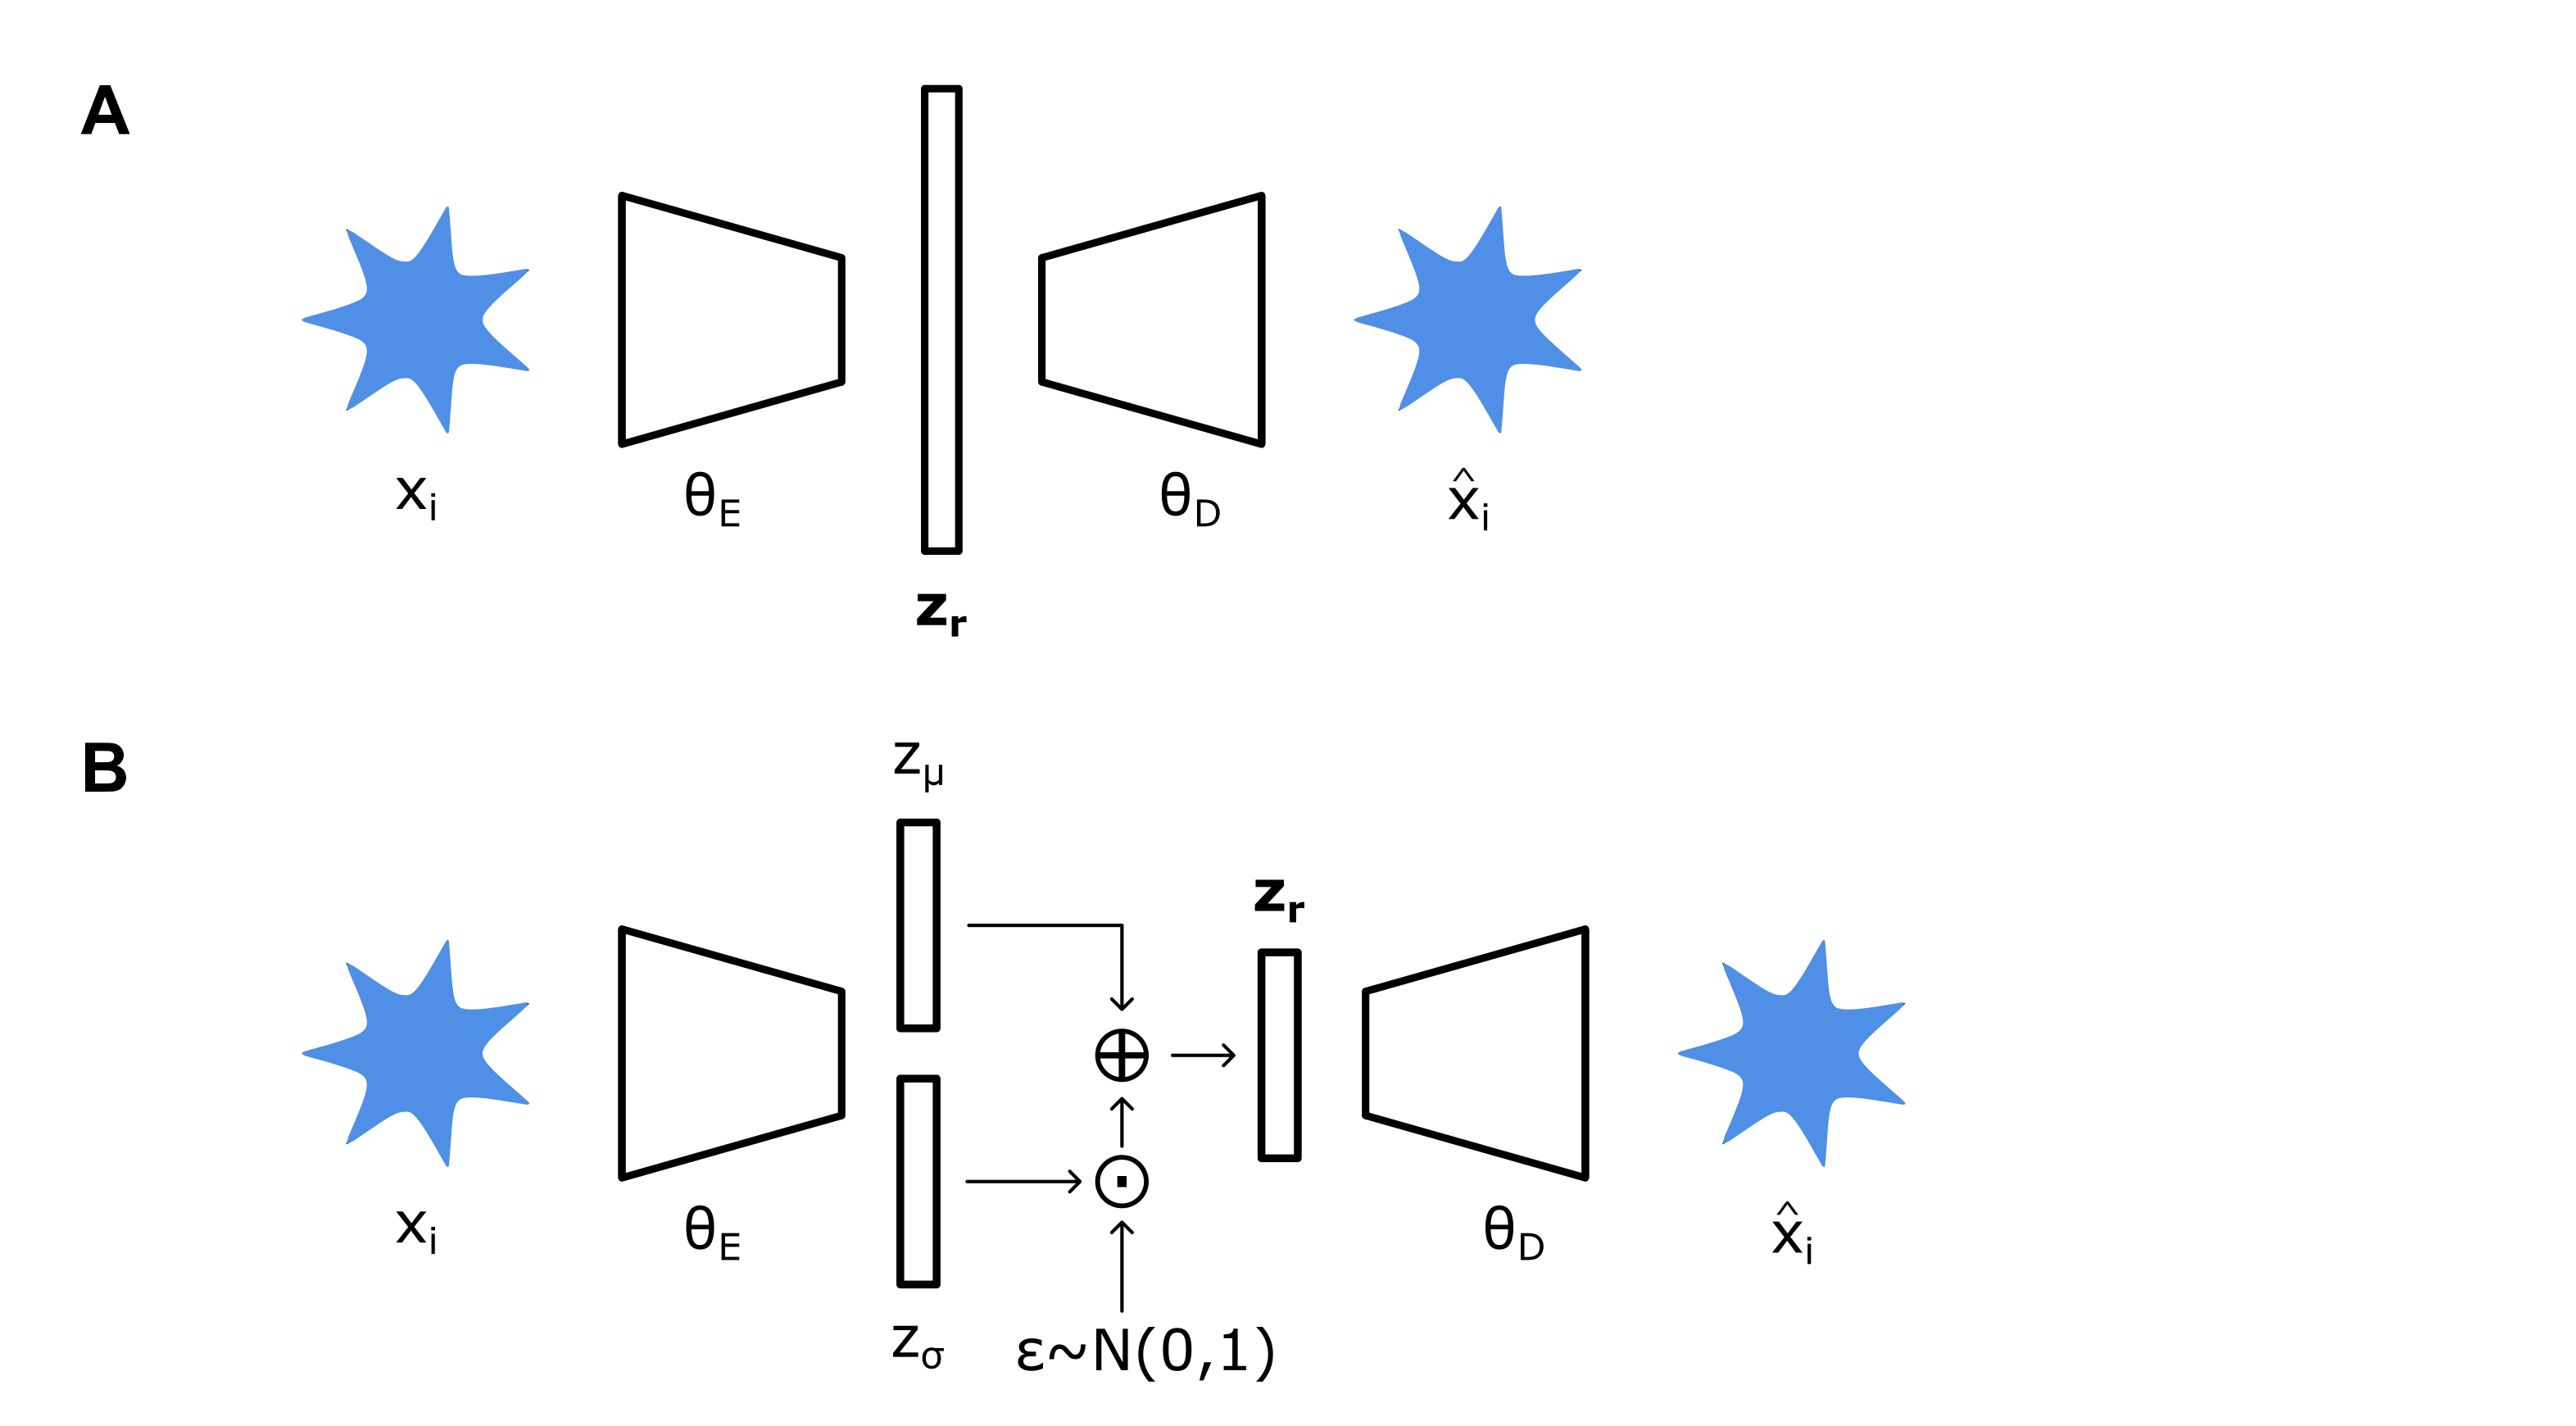
\includegraphics[scale=0.9]{fig4.png}
		\caption{\textbf{A)} Autoencoder structure consisting of an encoder ($\theta_{E}$) which translates an input image $x_{i}$ into a vector of latent variables $\mathbf{z_{r}}$. A decoder ($\theta_{D}$) then attempts to reconstruct input data $\hat{x}_{i}$ from $\mathbf{z_{r}}$. \textbf{B)} A variational autoencoder consists of similar components, however $\theta_{E}$ maps $x_{i}$ instead to deterministic parameters $z_{\mu}$ and $z_{\sigma}$ which describe a probabilistic distribution. These are then used to obtain $\mathbf{z_{r}}$ and similarly decoded.}
		\label{fig:fig4}
	\end{figure}
		
%	\begin{equation}
		\begin{align}
			\min \bm{\mathcal{L}}(\theta_{E}, \theta_{D}) &= \min_{\theta_{E}, \theta_{D}} \sum_{i=1}^{N} \mathcal{L}^{rec}(x_{i}, \hat{x_{i}}) \label{eq:autoencoder} \\ 
			\mathrm{where} \quad \hat{x_{i}} &= \theta_{D}(\theta_{E}(x_{i})) \nonumber
        \end{align}
%	\end{equation}
	
	\begin{equation}
		\mathcal{L}^{rec}(x, \hat{x}) = \vert\vert x - \hat{x} \vert\vert_{2}^{2}
		\label{eq:l2norm}	
	\end{equation}

	Latent variables $\bm{z_{r}}$ in a standard AE configuration are, in principle, unstructured. Thus, sampling new data in generative processes might not lead to valid data as the properties and ranges of $\bm{z_{r}}$ values are not known. Appending regularization terms, $\mathcal{L}^{reg}(\bm{z_{r}})$, to the cost function (Equation \ref{eq:autoencoder}) can lead to more structured latent variables and the spaces they inhabit (Equation \ref{eq:regautoencoder}). These modified AE structures are, thus, referred to as regularized autoencoders \cite{Ehrhardt2022}. 
	
%	\begin{equation}
		\begin{align}
			\min \bm{\mathcal{L}}(\theta_{E}, \theta_{D}) &= \min_{\theta_{E}, \theta_{D}} \sum_{i=1}^{N} \mathcal{L}^{rec}(x_{i}, \hat{x_{i}}) + \lambda \mathcal{L}^{reg}(\bm{z_{i}}) \label{eq:regautoencoder} \\ 
			\mathrm{where} \quad \hat{x_{i}} &= \theta_{D}(\theta_{E}(x_{i})) \nonumber
        \end{align}
%	\end{equation}
	
	$\lambda$ is a balancing term used to adjust the trade-off between latent-space regularity and reconstruction quality. On the other hand, $\mathcal{L}^{reg}(\bm{z_{r}})$, can take many forms and is detailed further elsewhere \cite{Ehrhardt2022, pmlr-v48-arpita16}. 
	
	A variation of AEs is variational autoencoders (VAEs) which are similar but treat encoding and decoding in a probabilistic manner (Figure \ref{fig:fig4}B)\cite{RezendeMohamed14}. Instead of directly mapping input data to latent variables, VAEs map input data to probabilistic distributions of their corresponding latent variables. Briefly, $\theta_{E}$ maps input data to deterministic parameters, mean $z_{\mu}(x)$ and standard deviation $z_{\sigma}(x)$, which describe an underlying probabilistic distribution (usually Gaussian) of the latent space. These deterministic parameters are then injected with stochasticity sampled from a fixed normal distribution, where $\odot$ denotes a Hadamard product (Equation \ref{eq:vae}). This configuration is necessary to preserve the stochasticity within the latent space while enabling gradient-based backpropagation during training \cite{Ehrhardt2022}. In turn, the loss function (Equation \ref{eq:autoencoder}) is now modified to consider both reconstruction quality and regularity of the latent space (Equation \ref{eq:vaeloss}). The latter is usually represented by a Kullback–Leibler divergence, detailed elsewhere \cite{Ehrhardt2022}. Overall, a probabilistic treatment of latent variables and the spaces they inhabit leads to more structured, compact, and continuous latent spaces. This, in turn, leads to a smoother sampling of latent variables for generative processes and representation learning in general. 
	
	\begin{equation}
		z = z_{\mu}(x) + z_{\sigma}(x) \odot \epsilon \quad   \mathrm{with} \ \epsilon \sim \mathcal{N}(0,1)	
		\label{eq:vae}
	\end{equation}
	
	\begin{equation}
		\mathcal{L}^{VAE} = \mathcal{L}^{rec} + \mathcal{L}^{KL}
		\label{eq:vaeloss}
	\end{equation}
		
	AEs, VAEs, and variations thereof have many applications in generative frameworks and tasks involving reduced dimension representations of high dimensional data such as images. The strengths of these architectures in modeling complex data within low-dimensional representations could lend themselves well to capturing the complex nonlinearities inherent in longitudinal datasets. Mouches \textit{et al.} utilizes an invertible latent space disentanglement module within an autoencoder framework to determine latent variables that affect age-related changes \cite{pmlr-v143-mouches21a}. Isolated age-related latent variables can then be varied, with age-unrelated components kept constant, to simulate the aging of a particular individual. Following a similar vein, Zhao \textit{et al.} utilized a cosine-based loss function to disentangle brain age from image representation \cite{Zhao2021}. They did so with a self-supervised learning methodology, optimizing the correspondence between the 'directionality' of latent variables in the latent space and physical developmental trajectories. Sauty and Durrleman utilized a VAE to learn latent variables representing images within a longitudinal dataset \cite{Sauty2022}. These latent variables are then fitted to a linear longitudinal mixed-effects progression model similar to those of the LDDMM framework.  
	
	Overall, AEs and VAEs represent powerful tools for reducing high-dimensional data into a low-dimensional latent space, efficiently encapsulating longitudinal data into compressed latent variables. Nevertheless, the problem remains with the underlying physical significance of latent variables and latent spaces, or the lack thereof \cite{Ehrhardt2022}. Latent variables and their spaces are solely reduced dimension representations of the original input data; latent variables have no underlying physical meaning. For example, the distribution of latent variables has been shown to be affected by training parameters, demonstrating their capricious nature \cite{Lapenda2020}. Thus, latent variables cannot be considered spatiotemporal variables. However, rational structuring and regularization to ensure that latent spaces are enriched with physical meaning can lead to better outcomes. Another point of concern is that both AEs and VAEs generally treat latent spaces and variables in a Euclidean manner, when in fact research has shown that a manifold-based approaches may be more prudent \cite{pmlr-v130-connor21a}. These problems remain active fields of research, with solutions such as regularization and explicitly structuring latent spaces deterministically being continually developed \cite{yeyeyeyeye, ghosh2020from}. Nonetheless, existing works for spatiotemporal shape modeling demonstrated the potential applicability for autoencoders and learned latent variables to model longitudinal trajectories.	
	
	\subsection{Generative Adversarial Networks}
				
		Generative Adversarial Networks (GANs) are neural network architectures first proposed by Goodfellow \textit{et al.} \cite{NIPS2014_5ca3e9b1}. In principle, they consist of generator $\theta_{G}$ and discriminator $\theta_{Dsc}$ networks being trained simultaneously (Figure \ref{fig:fig5}). Therein, the former is trained to create new synthetic images, whilst the latter is trained to detect if an image is real or fake. In detail, $\theta_{G}$ maps random input variables $\nu$ (sampled from a prior distribution $p(\nu)$) to the data space in an attempt to generate data $\hat{x}_{G}$ resembling data from a real dataset $x_{r}$. In turn, both types of data are fed into $\theta_{Dsc}$, whereby $\theta_{Dsc}$ is trained to determine if data is real or fake. The objective function used to train both networks simultaneously is then a minimax problem (Equation \ref{eq:GANminimax}).
				
		\begin{figure}
			\centering
			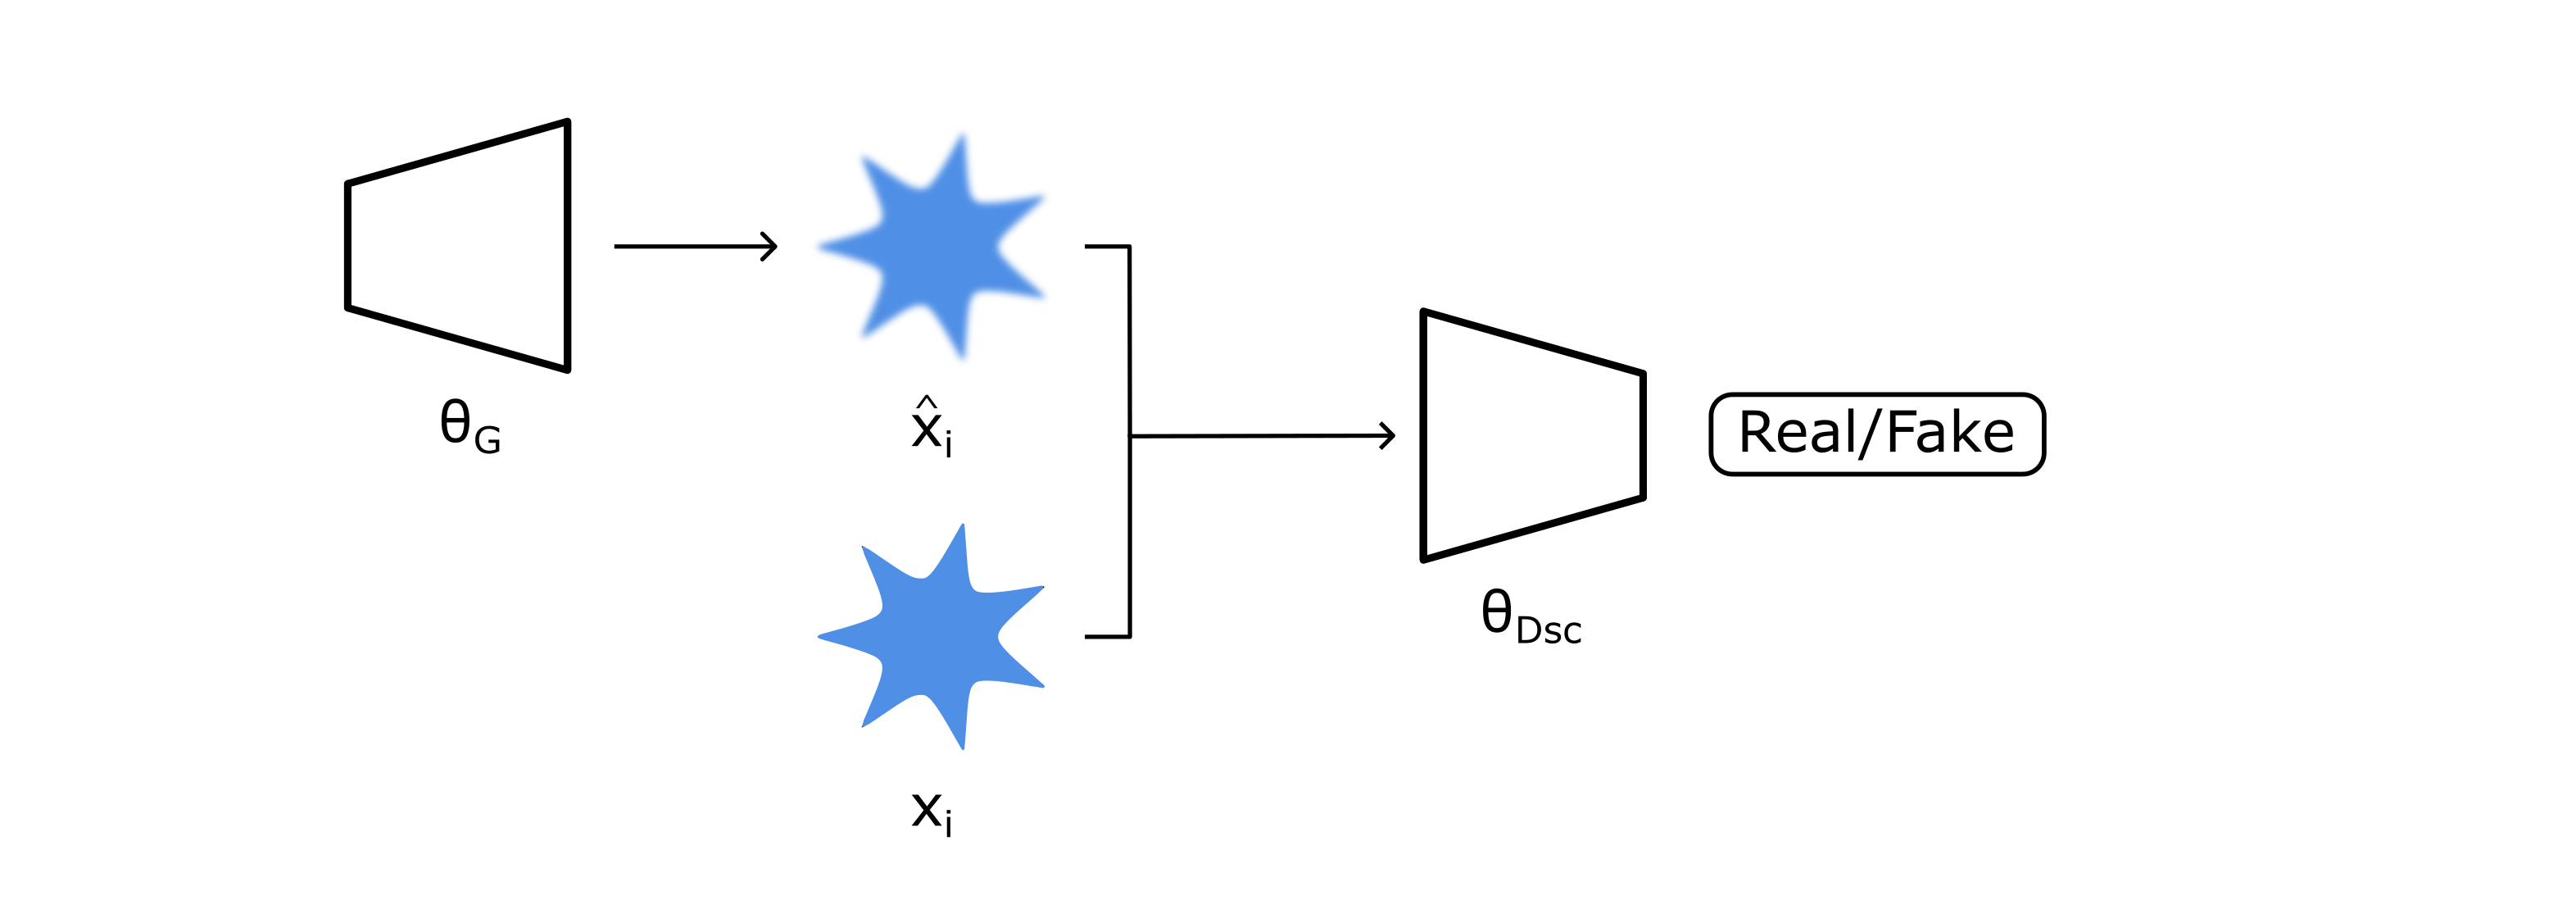
\includegraphics[scale=0.9]{fig5.png}
			\caption{A generative adversarial network (GAN) architecture consists of a generator ($\theta_{G}$) which creates synthetic data ($\hat{x}_{i}$) resembling real data ($x_{i}$). A discriminator ($\theta_{Dsc}$) then attempts to differentiate real versus 'fake' synthetic data. Both $\theta_{G}$ and $\theta_{Dsc}$ are jointly trained so that the former generates increasingly realistic images while the latter is able to discriminate real \textit{vs.} fake data better.}
			\label{fig:fig5}
		\end{figure}
		
		\begin{equation}
			\min_{\theta_{G}}\max_{\theta_{Dsc}} V (\theta_{G}, \theta_{Dsc}) = E_{x\sim p_{data}(x_{r})} [ \log D(x) ] + E_{z\sim p(\nu)} [ \log (1- D(G(\nu)))]
			\label{eq:GANminimax}
		\end{equation} 
		
		This architecture is very powerful, as the adversarial training configuration leads to the generator module being capable of generating realistic synthetic images that are indistinguishable from real data \cite{Wang2017, Gui2023}. Trained generators are then useful for many applications. In the context of medical imaging, examples include image synthesis, segmentation, and classification, among others \cite{Yi2019}. Many variants exist, and more are continually being developed, for which the reader is referred to other papers for further details \cite{Jabbar2021}. In the context of spatiotemporal shape modeling, GANs represent a powerful tool. Similar to previously discussed AEs and VAEs, their generative capacity can potentially be utilized to capture the underlying spatiotemporal trajectories. 
			
		Elazab \textit{et al.} used a stack of 3D GANs to predict brain tumor growth \cite{NL2016150352}. Specifically, with an input image and physiological feature maps, a generator predicted a brain scan at the proceeding time point whose accuracy was evaluated by a discriminator. Their results outperformed contemporary methods but relied on stacking and training consecutive GANs, which is computationally inefficient. Alternatively, Zhang \textit{et al.} utilized GANs to uncover the underlying data manifold of longitudinal progression for face aging \cite{zhang2017age}. They first encode images to latent vectors, which are concatenated with age-related feature vectors and then mapped onto a manifold. Discriminators ensure regularized latent vector generation and image realism of the generators. Based on this, Ravi \textit{et al.} developed a 2D framework to model age-related brain degeneration in the context of Alzheimer's diagnosis \cite{RaviAlex2019}. They incorporated further voxel-based and region-level constraints which acted as biological constraints to model Alzheimer's progression, leading to improved prognoses. They developed this work further to examine 3D MRIs for a more holistic view of the brain \cite{Ravi2022}. Utilizing a 3D training consistency mechanism and a super-resolution module led to a full 4D model of brain aging without a loss in anatomical detail. Following the same principle of temporal embedding within a latent space, Schön \textit{et al.} similarly implemented a GAN-based network for embedding temporal directionality in generators \cite{SchonSelvan23}. Alternative GAN architectures have also been investigated. Wasserstein GANs (WGANs) utilize Wasserstein distances as a loss function as opposed to regularly used Jensen-Shannon divergence \cite{pmlr-v70-arjovsky17a}. This architecture leads to more stable training outcomes and was utilized by Wegmayr \textit{et al.} as a recursive generator model to predict time steps in brain aging \cite{Wegmayr2019}. Combined with a classifier network, they present a framework for both predicting aged brain images and Alzheimer's prognosis, outperforming standard methods. In StyleGAN and derivatives thereof, the principle of style transfer and additional, intermediate latent spaces is utilized to improve generator architectures and disentangle latent space components and their effects on synthesized images \cite{Karras_2019_CVPR, Karras_2020_CVPR, Fetty2020}. Han \textit{et al.} developed a framework for image-based osteoarthritis prognosis using StyleGAN as the generative architecture \cite{Han2022}. This enabled them to construct the underlying manifold of longitudinal knee aging, and furthermore, they demonstrated that their model outperforms human radiologists in early diagnosis of osteoarthritis. Similarly, Gadewar \textit{et al.} utilized StarGAN-v2, a similar style-based generator architecture, to predict aging in structural MRIs of the brain \cite{Gadewar2023, Gadewar2023a}. 

		In short, GAN-based architectures and adversarial training represent powerful tools for spatiotemporal shape modeling. In particular, discriminators support the structuring and regularization processes so that the latent space of generator modules is physically meaningful, similar to previously discussed regularized AEs. While GANs have their own challenges in terms of training stability, mode collapse, convergence, and image fidelity, continual developments in training schemes, architectures, and loss functions have led to continuous improvements \cite{Yi2019, Gui2023, Saxena2021}. Generators with well-defined and structured latent spaces and rational generative processes enable us to predict growth trajectories. Said structuring of latent spaces is facilitated by discriminators and loss functions, which allow us to ensure smooth latent spaces that are temporally consistent and valid. In essence, in helping structure latent spaces, discriminators implicitly define the underlying manifold of spatiotemporal shape progression. Similar to previously discussed AEs, this structuring process ensures that latent spaces and variables therein can be endowed with meaningful physical characteristics.   			

	\subsection{Recurrent Neural Networks}
	
		Recurrent neural networks (RNNs) are a type of NN that are used to model sequential data such as a time series \cite{Lipton2015, Salehinejad2018, Staudemeyer2019}. They do so by considering data along a whole sequence's trajectory during training and inference; RNNs are designed explicitly with features that connect and consider data inputs across longitudinal sequences by maintaining memory (\textit{i.e.,} a hidden internal state $h_{t}$ which is continually updated at each time point $t$). Early RNNs utilized simple 'context units', which are units independently connected to nodes in the hidden layer of an NN (Figure \ref{fig:fig6}B) \cite{Elman1990}. These context units are then updated along steps in a data sequence \textit{via} activation functions as the RNN is trained along a sequence (Figure \ref{fig:fig6}A). To address practical issues regarding optimization of network parameters (exploding/vanishing gradients during backpropagation) \cite{Lipton2015, Salehinejad2018, Staudemeyer2019}, newer RNN architectures utilize complex memory cells instead of traditional nodes \cite{Hochreiter1997, Yu2019, Chung2014}. A prime example is the Long Short-Term Memory (LSTM) cell. These types of cells utilize 'gates', components that determine when and how to modify the memory of the cell (Figure \ref{fig:fig6}C). In detail, the three main gates of a standard LSTM cell are the forget, input, and output gates. The forget gate utilizes the output of the previous time point $y_{t-1}$ and the current input $x_{t}$ with a sigmoidal activation function to determine data in $h_{t}$ should be 'forgotten' (Equation \ref{eq:forgetgate}). Where $W$ and $b$ denote the weights and biases of the threshold units, respectively. 

		\FloatBarrier
		\begin{figure}
			\centering
			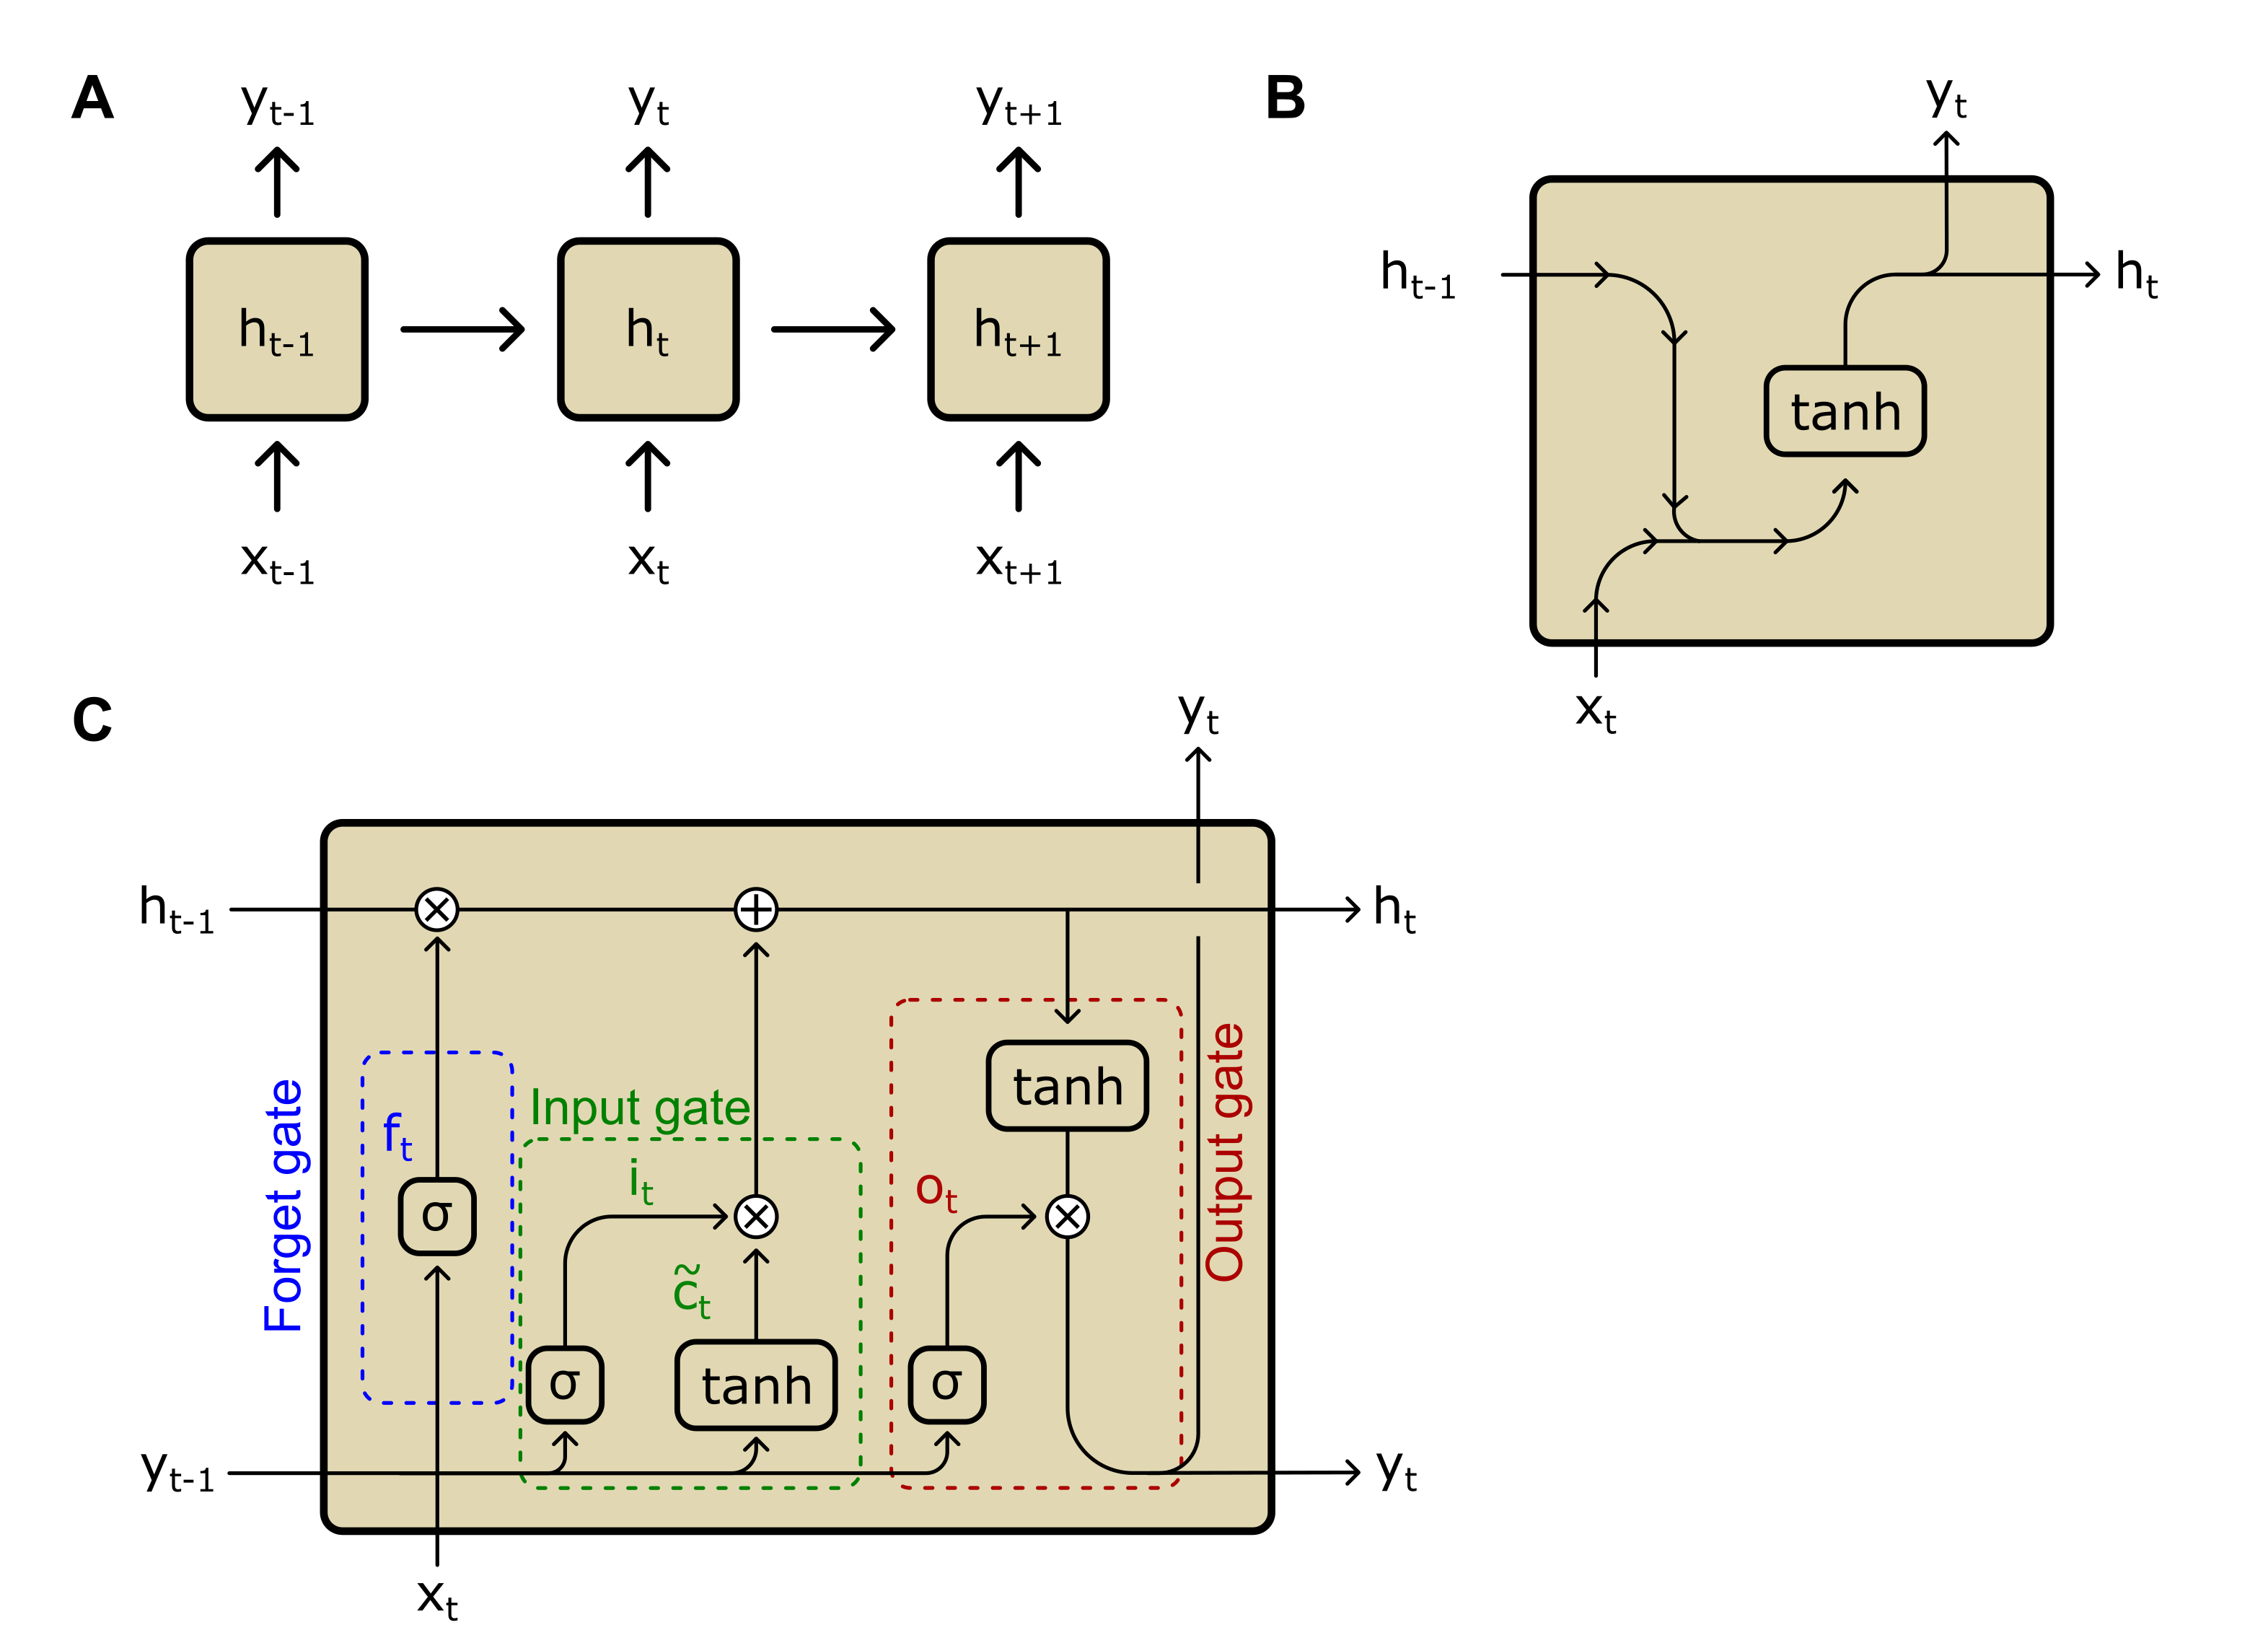
\includegraphics[scale=0.9]{fig6.png}
			\caption{\textbf{A)} A recurrent neural network (RNN) is trained along a sequence of time points $t$. Based on input ($x_{t}$) and output data ($y_{t}$), a hidden state ($h_{t}$) is continuously updated using context units. \textbf{B)} A simple context unit in early RNNs, wherein the input from the previous time point of the hidden state ($h_{t-1}$) is combined with $x_{t}$ and a $\tanh$ activation function to calculate $y_{t}$ and update $h_{t}$. \textbf{C)} A Long Short-Term Memory (LSTM) cell is a more complex unit used to maintain $h_{t}$ and determine $y_{t}$. Both sigmoidal ($\sigma$) and $\tanh$ activation functions are used within forget, input, and output gates, which determine which data is removed, added, and output from the cell. Figure inspired by existing work of \cite{45500}.}
			\label{fig:fig6}
		\end{figure}
		
		
		\begin{equation}
			f_{t} = \sigma(W_{f}[y_{t-1}, x_{t}] + b_{f})
			\label{eq:forgetgate}
		\end{equation} 
		
		Similarly, for the input gate, a sigmoidal activation function determines which values are to be updated (Equation \ref{eq:lstmit}), and a $\tanh$ activation function creates new values to be added to the internal state (Equation \ref{eq:lstmtanh}).   
		
		\begin{equation}
			i_{t} = \sigma(W_{i}[y_{t-1}, x_{t}] + b_{i})
			\label{eq:lstmit}
		\end{equation}
		
		\begin{equation}
			\tilde{c_{t}} = \tanh (W_{c}[y_{t-1}, x_{t}] + b_{c})
			\label{eq:lstmtanh}
		\end{equation}
			
		Together, Equations \ref{eq:forgetgate} - \ref{eq:lstmtanh} are combined to update $h_{t}$, where $*$ denotes pointwise multiplication (Equation \ref{eq:lstminternalupdate}).
		
		\begin{equation}
			h_{t} = f_{t} * h_{t-1} + i_{t} * \tilde{c_{t}}
			\label{eq:lstminternalupdate}
		\end{equation} 
			
		Finally, the output is determined by the output gates using $x_{t}$ and $y_{t-1}$ (Equation \ref{eq:lstmoutput1}) and $h_{t}$ (Equation \ref{eq:lstmoutput2}). 
		
		\begin{equation}
			o_{t} = \sigma ( W_{o}[y_{t-1}, x_{t}] + b_{o})
			\label{eq:lstmoutput1}
		\end{equation}
		
		\begin{equation}
			y_{t} = o_{t} * \tanh (h_{t})
			\label{eq:lstmoutput2}
		\end{equation}
			
		Thus far, LSTMs have been used for natural language processing or other tasks examining relatively low-dimensional data. In the context of images and CNNs, LSTMs have been adapted for image inputs in the form of the convolutional LSTM (ConvLSTM) \cite{NIPS2015_07563a3f}. ConvLSTM is able to capture temporal information and dependencies in a sequence of images while ensuring that spatial information is preserved during encoding. This has led to its use and marked effectiveness in video prediction tasks \cite{Lotter2016, Lu2017}. 
		
		In the context of longitudinal medical imaging, RNNs have improved the outcomes of segmentation \cite{Gao2018} and disease stage classification tasks \cite{Santeramo2018, Gao2018a, Cui2019, Ouyang2021, Ding2023}. In explicitly modeling shape change using ConvLSTMs and its derivatives, however, RNNs have seen comparatively less uptake potentially due to the significantly high GPU memory requirements \cite{MaZhangLiu22}. Some studies nevertheless utilize RNNs as components within larger frameworks to avoid this obstacle. For example, Pathan and Hong used LSTMs to predict the vector momentum sequences to deform a longitudinal baseline image in an LDDMM framework \cite{SharminYi18}. This approach leverages the effectiveness of the LDDMM framework to predict changes over time without loss of detail and the computational efficiency of DL. Louis \textit{et al.} utilized RNNs to encode longitudinal trajectories into a latent space \cite{Louis2019}. These encoded trajectories are then decoded to construct the manifold and the Riemannian metrics lying on this manifold. Ma \textit{et al.} utilized ConvLSTMs alongside a transformer in a 'growth prediction module' to predict tumor growth \cite{Ma2023}. They demonstrated that utilizing both components in a unified module leads to better-predicted growth morphologies. Zhang \textit{et al.} extended the ConvLSTM framework with the goal of modeling spatiotemporal sequences (ST-ConvLSTM) \cite{Zhang2020}. Their ST-ConvLSTM units learn both temporal and spatial dependencies in a sequence; for a 3D image slice, ST-ConvLSTM learns both the changes over time for that slice and accounts for the adjacent slices. 
		
		To surmise, RNNs represent a powerful network architecture for capturing temporal dependencies within a longitudinal dataset. Nevertheless, the issue of high GPU memory requirements for imaging data persists. This particular requirement precludes the use of RNNs for longitudinal shape modeling. Nevertheless, Ma \textit{et al.} sought to address this by developing multi-scale RNN frameworks, which demonstrably improve performance with much lower GPU memory costs \cite{MaZhangLiu22, Ma2023a}. Chen \textit{et al.} demonstrated the use of signed distance function-based representations with ConvLSTMs to predict longitudinal changes in the shape of vestibular schwannoma \cite{ChenWolterJelmerNeve2024}. They demonstrated a proof of concept for using signed distance functions, which could address issues of large memory requirements of conventional ConvLSTMs operating directly on images. All in all, developments in using LSTMs for medical imaging datasets are relatively recent and have yet to be fully investigated in the context of longitudinal medical image shape modeling. 
	
	\subsection{Transformers}
		
		Transformers are a relatively recent development in DL. Originally designed for natural language processing (NLP) tasks \cite{Vaswani2017}, they utilize a novel attention mechanism based on saliency, which can capture long-range dependencies in data sequences. The architecture was later developed further specifically for image data with the Vision Transformer (ViT) framework \cite{Dosovitskiy2020}. In any case, transformer networks rely firstly on tokenization of input data \cite{Shamshad2023, Islam2024, Torralba2024-ce}. For text data, tokenization is relatively straightforward, but for images, the ViT framework relies on patching, a process to divide a larger image into $N$ smaller fixed-sized patches. These image patches are then linearly projected and embedded alongside their positions to encode the relative positions of each patch. These embedded patch and position data represent and thus are token representations of the original image data $\mathbf{T} = [t_{i},..., t_{N}]$ (Figure \ref{fig:fig7}). These tokens are then passed to attention models,  where 'query' $\mathbf{q}$, 'key' $\mathbf{k}$, and 'value' $\mathbf{v}$ vectors for each token are calculated by their respective projection matrices ($W_{q}, W_{k}, W_{v}$) (Equation \ref{eq:qkv}). These vectors are then compiled into larger matrices $\mathbf{Q}, \mathbf{K}, \mathbf{V}$ respectively (Equation \ref{eq:qkv}). 
		
		\FloatBarrier
		\begin{figure}
			\centering
			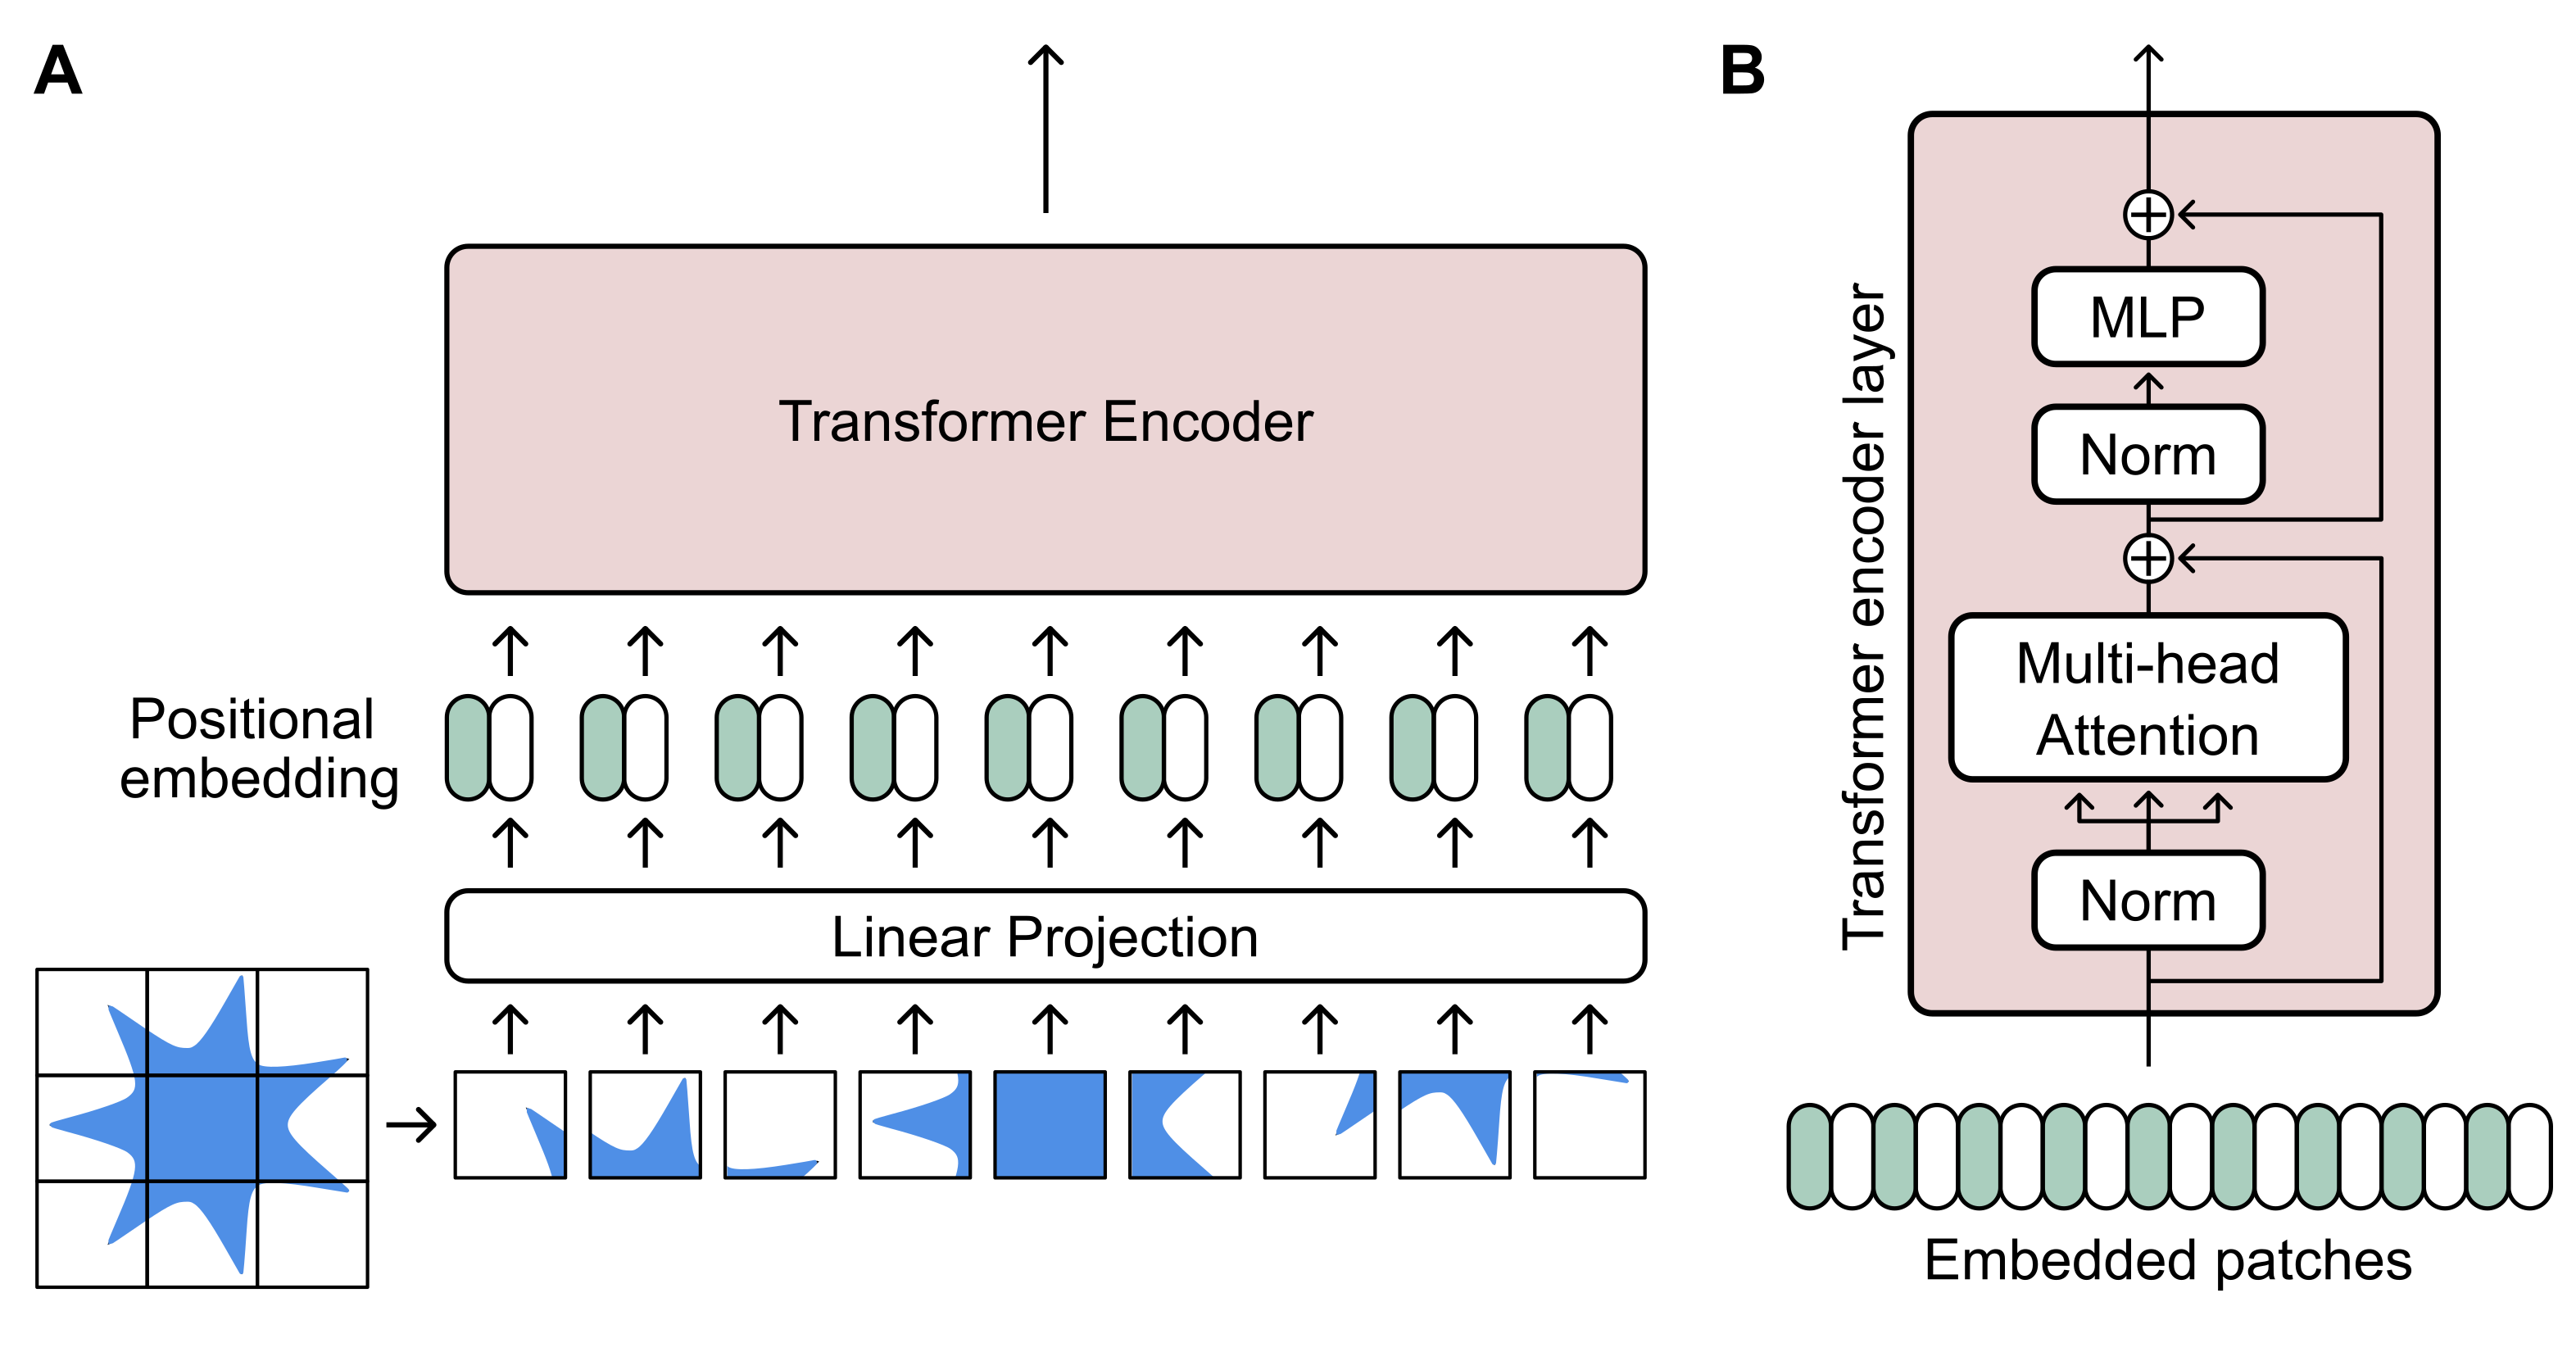
\includegraphics[scale=0.9]{fig7.png}
			\caption{\textbf{A)} A Visual Transformer (ViT) architecture tokenizes an input image by first delineating it into smaller patches. Each patch is then linearly projected and embedded alongside its positional data before being fed into a transformer encoder. \textbf{B)} A transformed encoder layer takes the embedded image patches as tokens and uses them within a multi-head attention-based encoder layer. Figure inspired by existing work of \cite{Dosovitskiy2020}.}
			\label{fig:fig7}
		\end{figure}

%		\begin{equation}
			\begin{align}
				\mathbf{Q} &= 
				\begin{bmatrix}
					\mathbf{q}_{1}^{\top}\\
					\vdots \\ 
					\mathbf{q}_{N}^{\top}
				\end{bmatrix} = 
				\begin{bmatrix}
					(W_{q}t_{1})^{\top}\\
					\vdots \\ 
					(W_{q}t_{N})^{\top}
				\end{bmatrix} = \mathbf{T} \mathbf{W}_{q}^{\top} \nonumber \\ 
				\mathbf{K} &= 
				\begin{bmatrix}
					\mathbf{k}_{1}^{\top}\\
					\vdots \\ 
					\mathbf{k}_{N}^{\top}
				\end{bmatrix} = 
				\begin{bmatrix}
					(W_{k}t_{1})^{\top}\\
					\vdots \\ 
					(W_{k}t_{N})^{\top}
				\end{bmatrix} = \mathbf{T} \mathbf{W}_{k}^{\top} \label{eq:qkv} \\ 			
				\mathbf{V} &= 
				\begin{bmatrix}
					\mathbf{v}_{1}^{\top}\\
					\vdots \\ 
					\mathbf{v}_{N}^{\top}
				\end{bmatrix} = 
				\begin{bmatrix}
					(W_{v}t_{1})^{\top}\\
					\vdots \\ 
					(W_{v}t_{N})^{\top}
				\end{bmatrix} = \mathbf{T} \mathbf{W}_{v}^{\top}\nonumber 
			\end{align}
%  		\end{equation}
		
		
		These vectors are then used to calculate an attention score which represents the saliency of the tokens $\mathbf{T}_{out}$ in an architecture referred to as self-attention (Equation \ref{eq:selfattention}), where $\sqrt m $ is a scaling factor based on the dimensionality of $\mathbf{K}$ to ensure stability during training.
		
		\begin{equation}
			\mathbf{T}_{out} = \mathrm{softmax} \left(\frac{\mathbf{Q}\mathbf{K}^{\top}}{\sqrt m} \right) \mathbf{V}
			\label{eq:selfattention}
		\end{equation}
		
		However, self-attention is relatively limited and, instead, multi-head self-attention (MHSA) is able to better capture map saliency and capture context. Essentially, MHSA has $n$ parallel self-attention layers, each with their own learned projection matrices $\mathbf{W}_{q,i}, \mathbf{W}_{k,i}, \mathbf{W}_{v,i}$. Outputs from each layer are concatenated and projected using a learned output projection matrix $\mathbf{W}_{o}$ (Equation \ref{eq:multihead}). 
		
%		\begin{equation}
			\begin{align}
				&\mathbf{T}_{out,multi}	= \mathrm{concat}(\mathbf{T}_{out,1}, ..., \mathbf{T}_{out,n}) \mathbf{W}_{o} \label{eq:multihead}\\
				\mathrm{where} \quad &\mathbf{T}_{out,i} = \mathrm{softmax} \left(\frac{\mathbf{Q}_{i}\mathbf{K}_{i}^{\top}}{\sqrt m} \right) \mathbf{V}_{i} \nonumber \\ 
				\mathrm{and} \quad 	\mathbf{Q}_{i} &= 
				\begin{bmatrix}
					\mathbf{q}_{1,i}^{\top}\\
					\vdots \\ 
					\mathbf{q}_{N,i}^{\top}
				\end{bmatrix} = 
				\begin{bmatrix}
					(W_{q,i} \; t_{1})^{\top}\\
					\vdots \\ 
					(W_{q, i} \; t_{N})^{\top}
				\end{bmatrix} = \mathbf{T} \mathbf{W}_{q,i}^{\top} \nonumber \\ 
				\mathbf{K}_{i} &= 
				\begin{bmatrix}
					\mathbf{k}_{1,i}^{\top}\\
					\vdots \\ 
					\mathbf{k}_{N,i}^{\top}
				\end{bmatrix} = 
				\begin{bmatrix}
					(W_{k,i} \; t_{1})^{\top}\\
					\vdots \\ 
					(W_{k,i} \; t_{N})^{\top}
				\end{bmatrix} = \mathbf{T} \mathbf{W}_{k,i}^{\top} \nonumber \\ 			
				\mathbf{V}_{i} &= 
				\begin{bmatrix}
					\mathbf{v}_{1, i}^{\top}\\
					\vdots \\ 
					\mathbf{v}_{N, i}^{\top}
				\end{bmatrix} = 
				\begin{bmatrix}
					(W_{v,i} \; t_{1})^{\top}\\
					\vdots \\ 
					(W_{v,i} \; t_{N})^{\top}
				\end{bmatrix} = \mathbf{T} \mathbf{W}_{v,i}^{\top} \nonumber
            \end{align}
%		\end{equation}		
		
		These tokenized representations and attention modules are then integrated into various NN architectures and can be configured for many applications, especially in medical image analysis \cite{Azad2024}. In particular, the capability to capture long-range dependencies and focus on salient features across long input sequences could potentially be applicable for predicting shape changes over time sequences. 
		
		In the context of longitudinal shape modeling, the use of transformers are still relatively unexplored. Sarasua \textit{et al.} was one of the first to apply transformers to model longitudinal shape trajectories \cite{Sarasua2021}. They forecasted the change in the shape of meshes of the left hippocampus in an encoder-decoder-style architecture utilizing a bidirectional transformer encoder. They extended this work further by explicitly embedding Alzheimer's cognitive impairment scores and utilizing pre-trained transformers \cite{Sarasua2022}. The latter method revolved around freezing most layers of a pre-trained transformer and fine-tuning it on a selected task to decrease the number of trainable parameters \cite{Lu2021}. The former method of embedding cognitive scores was also similarly utilized by Xia \textit{et al.} to synthesize longitudinal brain images \cite{Xia2021}. With an input baseline brain image, their transformer architecture embeds a health state and age progression to synthesize changes over time. To improve the quality of their predicted progressions, they trained their networks in an adversarial manner with additional loss functions to preserve subject identity. Wang \textit{et al.} developed a comprehensive transformer-based framework to predict tumor growth \cite{Wang2022}. Their so-called static-dynamic framework utilizes a transformer-based module to first encode and enhance high-level features of detected tumors. Then, a transformer-based growth estimation module is employed to predict growth based on the aforementioned extracted features. 
		
		Nonetheless, the transformer architecture is still in its relative infancy, with applications for predicting longitudinal shape trajectories still developing. Advances in transformer architectures, such as incorporating multi-scale convolutions for enhanced time-series prediction, could potentially be applied to imaging data as well \cite{Wang2023}. However, there are a number of caveats to the enhanced performance of transformer-based networks \cite{Li2023}. Firstly, the nature of the transformer architecture leads to lower degrees of inductive bias, necessitating larger amounts of training data for better performance. This could potentially be addressed with pre-training as demonstrated by Lu \textit{et al.} \cite{Lu2021}, but nevertheless remains a consideration. Furthermore, training transformer architectures is computationally expensive, requiring significant computing resources, especially if applied to 3D volumetric medical imaging. In fact, a relatively high number of studies in the field are focused on reducing this computational burden \cite{Xia2023}. This heightened computational resources required thus present a barrier, prohibiting widespread development and applications to new data. Early studies have already demonstrated promising results, and transformer architectures could present a future avenue for spatiotemporal shape modeling. 		
		